\documentclass{article}
\usepackage{graphicx}
\title{Estimating Markov Random Field Parameters for the model prior}
\author{DJ Canoli}
\date{2/5/2011}

\begin{document}
\section{Estimating Markov Random Field Parameters for the model prior}

When choosing the nature of the parameters of our Markov Random Field, we want to err on both sides of the musical generality/specificity argument.  For example, we designed one parameter that measures whether a note stays the same or changes (denoted within the model as $\beta$).  In comparison, we designated another parameter arbiter of the likelihood of a specific note movement (e.g. moving up a whole step on a standard Western scale) and aggregated all possible note movements within an instrument's four octave range.  Another parameter involved measured how close to the middle of an instrument's range a specific voiced note was (represented as $\alpha$).  A final set of parameters measured the tendencies of certain harmonies to appear within a score - for example, there should be different weights on consonant intervals such as major thirds versus dissonant intervals such as a half-step or a tri-tone (6 half-steps).  

Prototype Scores:
We found multiple MIDI quintet scores of different genres to incorporate into a cell array of prototypes with which to initialize our Markov Random Field prior learning process.  These ranged from classical brass quintets to five-part arrangements of popular tv theme songs, so that the diversity of compositional technique and harmony would provide a broader learning environment.

We employed a Metropolis-Hastings sampler to draw from the array of prototype scores, updating each of the parameters accordingly.  Further, using Contrastive Divergence, we were able to move the parameter estimates along towards convergence via gradient ascent, using the notion that the a single parameter's component of the gradient is proportional to the difference between the expectation of the log of the derivative with respect to that parameter over the original score data and that of the newly sampled score data.  Combining all parameters into a space $\Theta$, and moving along the gradient so as to minimize the energy function of the MRF, we have the update function:

\[\Theta_{t+1} = \Theta_t + \eta\nabla_{\Theta}\]

where $\eta$ is the set of learning rates for the parameters, determined experimentally, and

\[\nabla_{\Theta} = \langle\frac{\partial\log{f(x;\Theta)}}{\partial\Theta}\rangle_{X^0} - \langle\frac{\partial\log{f(x;\Theta)}}{\partial\Theta}\rangle_{X^s}\]

Contrastive divergence allows us to approximate the gradient for the parameters by iterating only a few times through the MCMC process, which speeds up computation considerably.  In the above equation, $X^s$ represents the sth iteration of sampling the data X.

Once the parameters have been estimated to the point of convergence, we set them as the prior and proceed to subsequent signal processing.

\begin{figure}
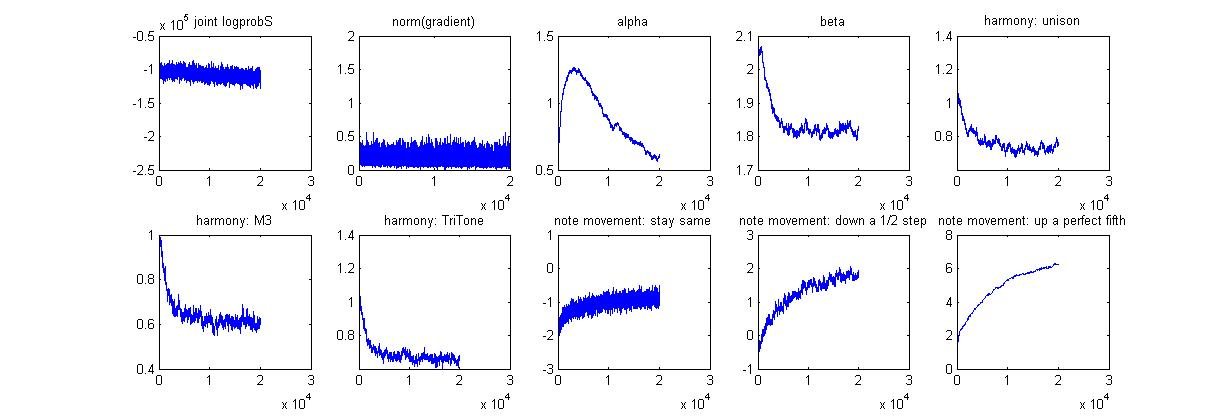
\includegraphics[height=40mm]{paramsnew(20000).jpg}
\end{figure}

\end{document}